\chapter{$\Lambda p$ event analysis}
In Sec. \ref{sec-multin}, the contribution of the multi-nucleon absorption processes was evaluated by using the $\Lambda p$ event distribution in the $K\otimes {\rm CDH}^{2 hits}$ trigger data. Here, the $\Lambda p$-event selection and the normalization factors for an evaluation of the yields of the $\Lambda p$ events are described.
\section{Event selection}
In order to reconstruct a pair of $\Lambda p$, one $\pi^-$ and two protons were required to be detected with the CDS. Events with more than 3 tracks were discarded. The two protons were checked whether either of them can reconstruct $\Lambda$ with the $\pi^-$.  Figure \ref{fig-lpselection}(left) shows the correlation of the two $p\pi^-$ invariant masses with each proton. The distance of closest approaches (DCAs) between the beam track and the reconstructed $p\pi^-$ parent track to discriminate the proton from the $\Lambda$ decay and the $p_1\pi^-$ pair was defined to give shorter DCA than the $p_2\pi^-$ pair. Although the $p_1\pi^-$ pair is naively expected to be more likely to be $\Lambda$ origin, the $p_2\pi^-$ pairs also contains $\Lambda$s  as a horizontal line is seen in Fig. \ref{fig-lpselection}(left). Therefore, the $p\pi^-$ pair whose invariant mass was closer to the $\Lambda$ mass was selected as a $\Lambda$ candidate and filled in Figure \ref{fig-lpselection}(right). The $\Lambda$ and side-band regions are also defined in Figure \ref{fig-lpselection}(right). The signal-to-noise ratio at the $\Lambda$ peak was approximately 5. Figure \ref{fig-lpinvmm} shows $^3$He($K^-,\Lambda p)X$ missing-mass and $\Lambda p$ invariant-mass spectra compared with side-band events in $\Lambda$ selection.

\begin{figure}[]
\begin{center}
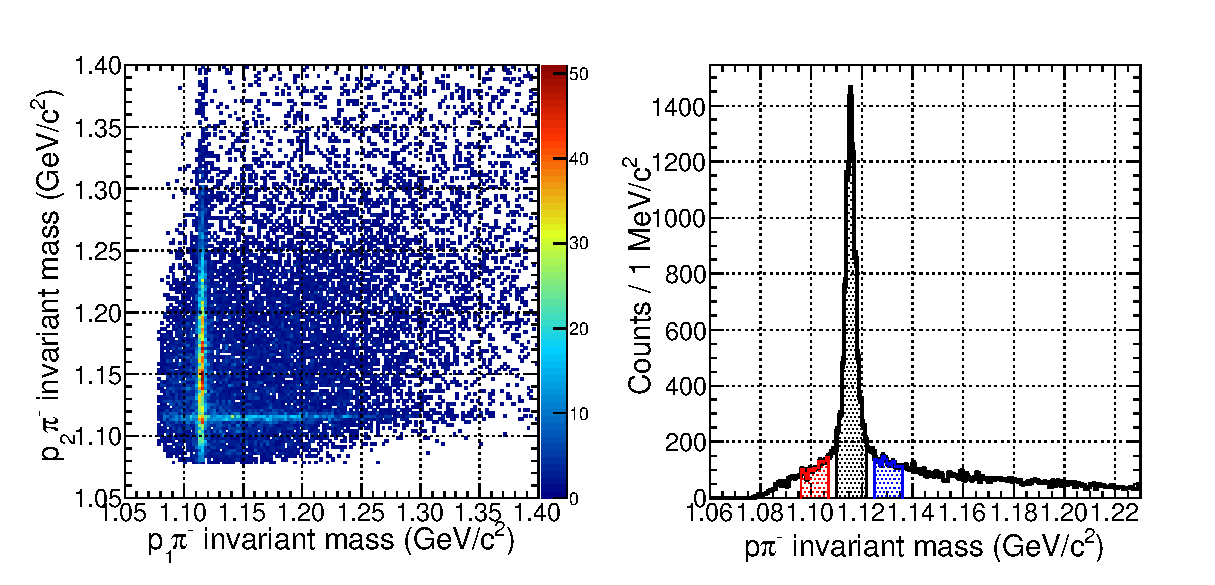
\includegraphics[width=\columnwidth]{./fig/lp_selection.eps}
\caption[Correlation of $p\pi^-$ invariant masses reconstructed with each proton in the $\pi^-pp$ events.]{(left) Correlation of $p\pi^-$ invariant masses reconstructed with each proton in the $\pi^-pp$ events. $p_1\pi^-$ has shorter DCA between the beam and reconstructed parent tracks than $p_2\pi^-$. (right) $p\pi^-$ invariant mass distribution in the $\pi^-pp$ events. The $p\pi^-$ pair whose invariant mass is closer to the $\Lambda$ mass is filled. The black hatched region represents $\Lambda$ selection, while blue and red hatches represent the side band regions.}
\label{fig-lpselection}
\end{center}
\end{figure}  

\begin{figure}[]
\begin{center}
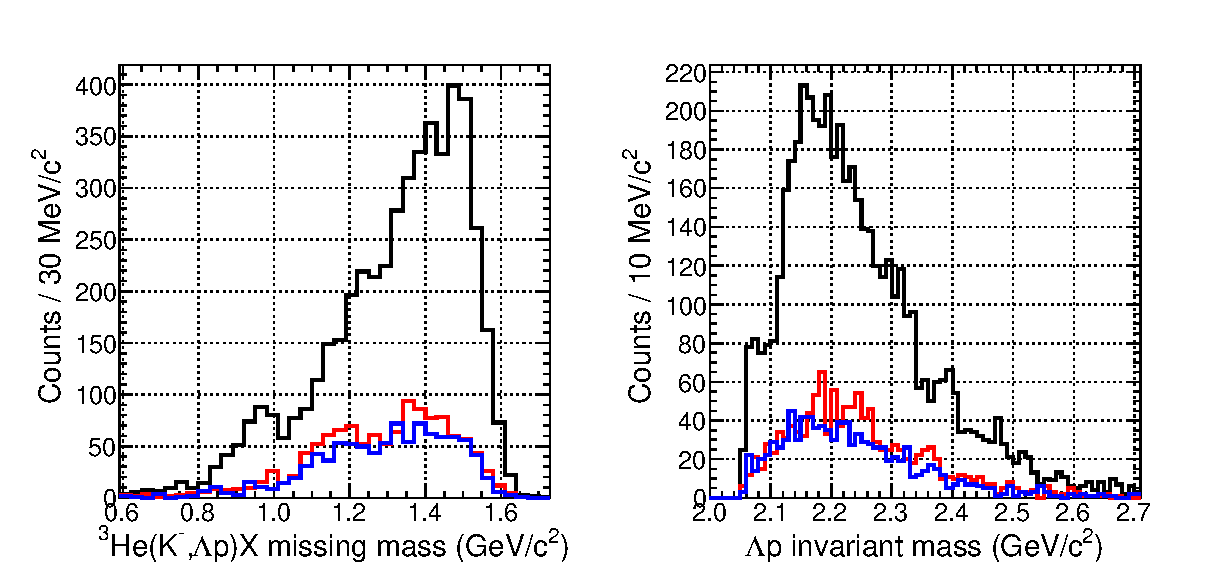
\includegraphics[width=\columnwidth]{./fig/lp_invmm.eps}
\caption[$^3$He($K^-,\Lambda p)X$ missing-mass and $\Lambda p$ invariant-mass spectra.]{(left) $^3$He($K^-,\Lambda p)X$ missing-mass and (right) $\Lambda p$ invariant-mass spectra. The blue and red histograms represent the side-band events in the $\Lambda$ selection as defined in Fig. \ref{fig-lpselection}.}
\label{fig-lpinvmm}
\end{center}
\end{figure}  

\section{Normalization}
The total cross-section of the $\Lambda p$ events can be expressed as,
\begin{eqnarray}
\sigma =\frac{1}{L}\cdot\frac{1}{\epsilon_{CDC}^3\cdot\epsilon_{PID}^3\cdot A'_{CDS}}\cdot\frac{1}{\epsilon'_{DAQ}\cdot\epsilon'_{trig}}\cdot N,
\end{eqnarray}
where $L$ and $\epsilon_{CDC}$ are the integrated luminosity and the CDC tracking efficiency, which are the same as those in Eq. \ref{eq-ncs}. $\epsilon_{PID}$ and $\epsilon'_{trig}$ are the efficiencies of the particle identification in the CDS and the $K\otimes CDH^{2 hits}$ trigger, which were assumed to be unity for the simplicity. $A'_{CDS}$ is the acceptance of the CDS to reconstruct three charged particles, $\pi^-pp$, evaluated by the simulation assuming phase-space uniform distribution of the multi-nucleon processes. $\epsilon'_{DAQ}$ is the live rate of the DAQ system with a consideration of the pre-scale factor of 7. These values are summarized in Table \ref{tab-lp}.

\begin{table}[]
\caption{Normalization factors for the $\Lambda p$ events.}
\begin{center}
\begin{tabular}{lc}
\hline\hline					
Luminosity $L$	($\mu$b$^{-1}$)	&	540					\\
$\epsilon_{CDC}$		&	0.96					\\
$\epsilon_{PID}$		&	1					\\
$\epsilon_{DAQ}'$		&	0.116					\\
$\epsilon_{trig}'$		&	1					\\
\hline\hline
\end{tabular}
\end{center}
\label{tab-lp}
\end{table}%


\section{$\Lambda pn$ final state}
It is worth mentioning that we can identify $\Lambda pn$ final state as a missing neutron peak in the $^3$He($K^-,\Lambda p)X$ missing-mass spectrum. If these events are attributed to NM2NA with a neutron spectator, we expect a corresponding peak around 2.8 GeV/$c^2$ in the $\Lambda p$ invariant-mass spectrum. No significant structure above 2.7 GeV/$c^2$ in Fig. \ref{fig-mmlpfit}(right) suggests that most of the $\Lambda pn$ events are attributed to 3NA. However, due to the limited statistics of the $\Lambda p n$ events, more detailed analysis cannot be achieved at present; we have obtained a few hundred $\Lambda p n$ events in the $^3$He$(K^-,\Lambda p)X$ missing-mass spectrum, in which only $\sim$ 10 events are available if we require the neutron to be detected with the NC. 
